\subsubsection{Messages and transactions}

As we said in \autoref{sec:accounts}, the accounts can send messages or
transactions to other accounts depending on the account's type.

A transaction is a single instruction constructed by an actor externally to the
scope of Ethereum \cite{wood2018ethereum}, it is serialized and included in the
blockchain. It can be used to transfer ether\footnote{The currency used within
Ethereum} or to trigger contract code. A transaction represents a message call
or the creation of a new account with associated EVM Code.

\begin{figure}[h]
  \centering
  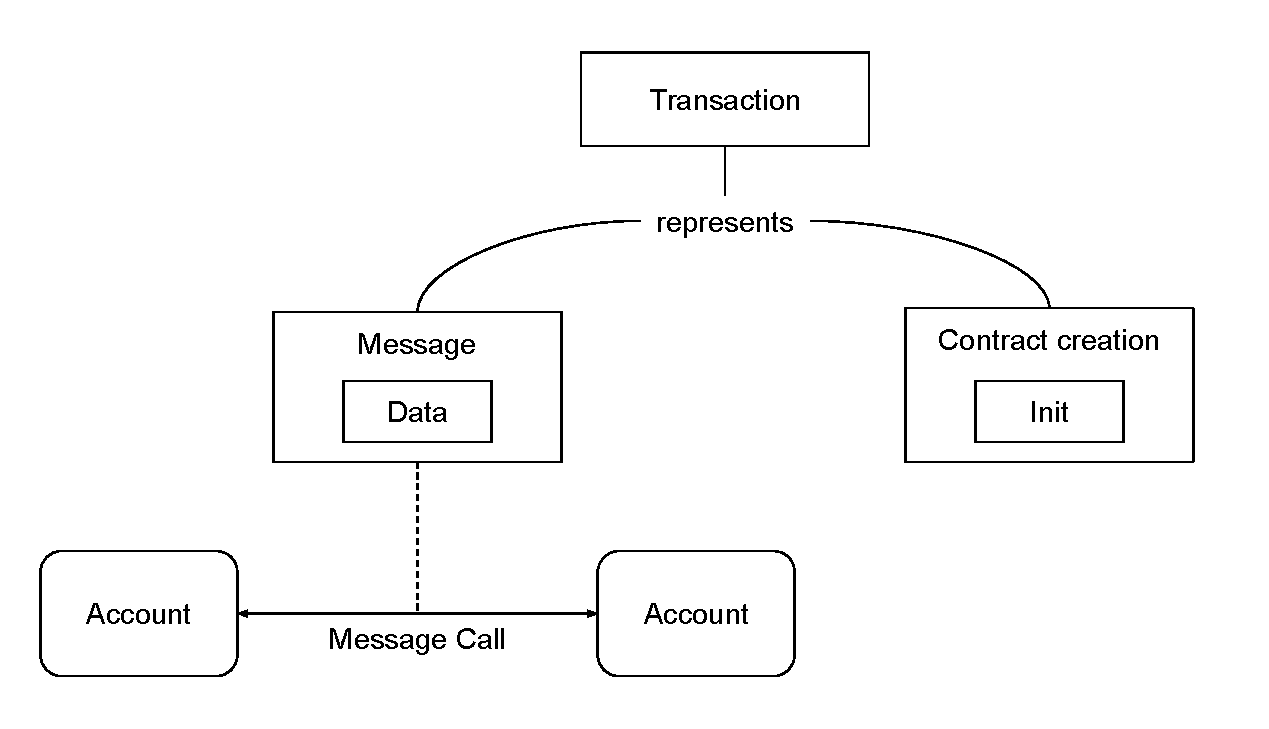
\includegraphics[width=0.9\textwidth]{./res/img/messages-transactions.pdf}
\caption{Representation of the relation between message and transaction.}
\label{fig:messages-transactions}
\end{figure}

A message is a virtual object that is not serialized and exists only in the
Ethereum execution environment. A message between two contract accounts is also
called \emph{internal transaction}, because of its dual nature of being
structured as a transaction and of being managed internally of the Ethereum
execution environment.

The relation between transactions, messages and contract creation is represented
in~\autoref{fig:messages-transactions}. We notice that messages and contract
creation have the same structure and both contain an unlimited size byte array.
The interpretation of this value depends on the type of transaction: if the
value is interpreted as \verb+data+, it represents the input for the message
call, else if it is interpreted as \verb|init|, it represents a piece of EVM
code used to initialize the storage of the smart contract and to return the EVM
code that will persist on the world state. We can distinguish the two types
of transaction depending on the receiver's address: if it is empty, it is a
contract creation, otherwise it is a message call.


\autoref{fig:messages-to-from-contract} shows the message call with regard to a
contract account. If the destination account is a contract, the message triggers
the execution of its code (\autoref{fig:messages-to-contract}). Instead, if the
message sender is a contract, the message is the result of the code execution
(\autoref{fig:messages-from-contract}).

\begin{figure}[t!]
  \centering
  \begin{subfigure}[t]{.4\textwidth}
    \centering
    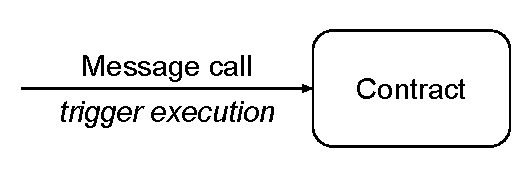
\includegraphics[width=\textwidth]{./res/img/messages-to-contract.pdf}
    \caption{Message call to a contract account which trigger the execution of code.}
    \label{fig:messages-to-contract}
  \end{subfigure}
  \hskip 3em
  \begin{subfigure}[t]{.4\textwidth}
    \centering
    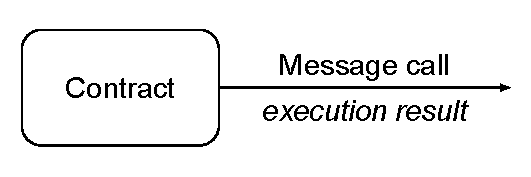
\includegraphics[width=\textwidth]{./res/img/messages-from-contract.pdf}
    \caption{Message call from a contract account which represents the result of code execution.}
    \label{fig:messages-from-contract}
  \end{subfigure}
  \caption{Message call to and from a contract account.}
  \label{fig:messages-to-from-contract}
  \end{figure}
